\begin{graphicspathcontext}{{./chapters/simulation/examples/imgs/},{./chapters/simulation/examples/imgs/auto/},\old}

\begin{frame}{Highway Simulation}
	\begin{block}{What is simulated?}
		\begin{enumerate}
		\item Vehicles on a French highway.
		\item Danger event $\rightarrow$ ``an animal is crossing the highway and causes a crash''. 
		\item Alert events by GSM.
		\item Arrival of the security and rescue services.
		\end{enumerate}
	\end{block}
	\vfill
	\includegraphics[width=.6\linewidth]{uml_Aremis}\hfill\includegraphics[width=.25\linewidth]{voxelia2}
\end{frame}

\sidecite{GallandGaudDemangeKoukam2009_11}
\begin{frame}{Model of the Environment}
	\smaller
	\begin{block}{Road Network}
		\begin{itemize}
		\item Road polylines: $S = \left\{ \langle path, objects \rangle \big| path = \langle (x_0,y_0) \cdots \rangle \right\}$
		\item Graph: $G = \left\{ S, S \mapsto S, S \mapsto S \right\} = \left\{ \text{segments}, \text{entering}, \text{exiting} \right\}$
		\end{itemize}
	\end{block}
	\begin{block}{Operations}
		\begin{itemize}
		\item Compute the set of objects perceived by a driver (vehicles, roads...):
			\[P = \left\{ o \Bigg|
				\begin{matrix}
				distance(d,o)\le \Delta \wedge \\
				o \in O \wedge \\
				\forall (s_1,s_2), path = s_1.\langle p, O \rangle.s_2
				\end{matrix}
				\right\}\]
			where $path$ is the roads followed by a driver $d$
		\item Move the vehicles, and avoid physical collisions
		\end{itemize}
	\end{block}
\end{frame}

\begin{frame}[t]{{Driving} Model}
	\begin{columns}
		\begin{column}{.35\linewidth}
			\centering
			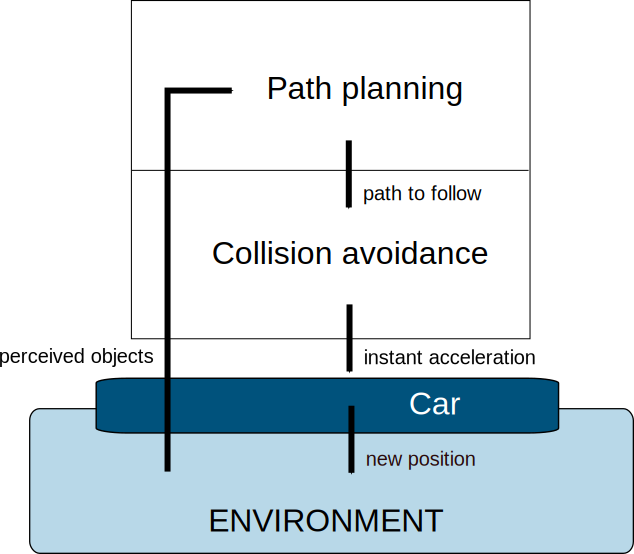
\includegraphics{carpooling_agent_layers}
			{\smaller\smaller\cite{GallandGaudDemangeKoukam2009_11}}
		\end{column}
		\begin{column}{.65\linewidth}
			\smaller
			\begin{block}{Path Planning}
			Based on the A* algorithm \cite{Dechter:1985:GBS:3828.3830,RoutePlanningAlgorithms2009} or D*-lite \cite{Koenig.Dstarlite.2005}
			\end{block}
			\begin{block}{Collision Avoidance}
				\begin{compactdescription}
				\item[Principle] compute the acceleration of the vehicle to avoid collisions with the other vehicles
				\item[Intelligent Driver Model] \cite{PhysRevE.62.1805}
				{\smaller
					\[acc = \begin{cases}
					- \dfrac{\left( v \Delta v \right)^2}{4b\Delta p^2} & \text{if the ahead object is far} \\
					- a \dfrac{\left( s + v w \right)^2}{\Delta p^2} & \text{if the ahead object is near} \\
					\end{cases}\]
				}
				\item[Free driving]
					{\smaller\[acc = a \left( 1 - \left(\frac{v}{v_c}\right)^4 \right)\]}
				\end{compactdescription}
			\end{block}
		\end{column}
	\end{columns}
\end{frame}

\begin{frame}[t,fragile]{Video of the French Highway Simulation}
	\vspace{-.25cm}
	\begin{center}
		\embeddedvideo[width=.8\linewidth]{./videos/simulation/aremis.avi}{aremis}
	\end{center}
	\begin{center}
		\tiny These videos were realized on the SIMULATE\textup{\regmark} tool \copyright Voxelia S.A.S
	\end{center}
\end{frame}

\end{graphicspathcontext}

\endinput

